\documentclass[11pt,compress,t,notes=noshow, aspectratio=169, xcolor=table]{beamer}

\usepackage{../../style/lmu-lecture}
% Defines macros and environments
% This file is included in slides and exercises

% Rarely used fontstyle for R packages, used only in 
% - forests/slides-forests-benchmark.tex
% - exercises/single-exercises/methods_l_1.Rnw
% - slides/cart/attic/slides_extra_trees.Rnw
\newcommand{\pkg}[1]{{\fontseries{b}\selectfont #1}}

% Spacing helpers, used often (mostly in exercises for \dlz)
\newcommand{\lz}{\vspace{0.5cm}} % vertical space (used often in slides)
\newcommand{\dlz}{\vspace{1cm}}  % double vertical space (used often in exercises, never in slides)
\newcommand{\oneliner}[1] % Oneliner for important statements, used e.g. in iml, algods
{\begin{block}{}\begin{center}\begin{Large}#1\end{Large}\end{center}\end{block}}

% Don't know if this is used or needed, remove?
% textcolor that works in mathmode
% https://tex.stackexchange.com/a/261480
% Used e.g. in forests/slides-forests-bagging.tex
% [...] \textcolor{blue}{\tfrac{1}{M}\sum^M_{m} [...]
% \makeatletter
% \renewcommand*{\@textcolor}[3]{%
%   \protect\leavevmode
%   \begingroup
%     \color#1{#2}#3%
%   \endgroup
% }
% \makeatother


\title{Interpretable Machine Learning}
% \author{LMU}
%\institute{\href{https://compstat-lmu.github.io/lecture_iml/}{compstat-lmu.github.io/lecture\_iml}}
\date{}

%\bibliography{feature-importance}
%\usepackage{Sweave}

%\usepackage{Sweave}
\begin{document}
	\newcommand{\titlefigure}{figure_man/feature-importance.png}
    \newcommand{\learninggoals}{
    	\item How SAGE fairly distributes importance
    	\item Definition of SAGE value function
    	\item Difference SAGE value function and SAGE values
    	\item Marginal and Conditional SAGE
    	}
	% Set style/preamble.Rnw as parent.
	
	% Load all R packages and set up knitr
	
	% This file loads R packages, configures knitr options and sets preamble.Rnw as 
	% parent file
	% IF YOU MODIFY THIS, PLZ ALSO MODIFY setup.Rmd ACCORDINGLY...
	
	% Defines macros and environments

	\lecturechapter{Shapley Additive Global Importance (SAGE)}
	\lecture{Interpretable Machine Learning}
	
	% ------------------------------------------------------------------------------

% CHALLENGE
\begin{frame}{Challenge: Fair Attribution of Importance}
\begin{columns}[T, totalwidth=\textwidth]
\begin{column}{0.54\textwidth}
\textbf{Recap:} 
\begin{itemize}
\item Data: $x_1, \dots, x_4$ uniformly sampled from $[-1, 1]$ 
\item DGP: $y:= x_1 x_2 + x_3 + \epsilon_Y$ with $\epsilon_Y \sim N(0, 1)$
\item Model: $\fh(x) \approx x_1 x_2 + x_3$
\end{itemize}

\lz

Although $x_3$ alone contributes as much to the prediction as $x_1$ and $x_2$ jointly, all three are considered equally relevant by PFI.
\end{column}
\begin{column}{0.45\textwidth}
\centering
  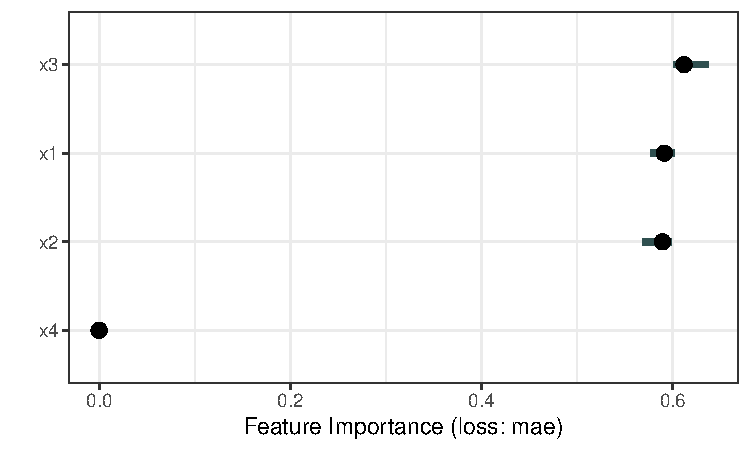
\includegraphics[width=\linewidth]{figure_man/pfi_interactions.pdf}
\end{column}
\end{columns}
\lz
\textbf{Reason:} PFI assesses importance given that all remaining features are preserved. If we first permute $x_1$ and then $x_2$, permutation of $x_2$ would have no effect on the performance (and vice versa).
\end{frame}



\begin{frame}{SAGE Idea \citebutton{Covert et al. (2020)}{https://proceedings.neurips.cc/paper/2020/file/c7bf0b7c1a86d5eb3be2c722cf2cf746-Paper.pdf}
}

\textbf{SAGE:} %Leverage game-theoretic 
Use Shapley values to compute a fair attribution of importance (via model performance)\\
\lz

\textbf{Idea:} 
\begin{itemize}
    \item Feature importance attribution can be regarded as cooperative game \\
    $\leadsto$ features jointly contribute to achieve a certain model performance
    \item Players: features
    \item Payoff to be fairly distributed: model performance
    \item Surplus contribution of a feature depends on the coalition of features that are already accessible by the model
\end{itemize}
%, where each feature is a player and model performance is the payoff. The surplus contribution of a feature depends on the coalition of features that are already in the room.\\
%\pause
\lz

\textbf{Note:} 
\begin{itemize}
    \item Similar idea (called SFIMP) was proposed in \citebutton{Casalicchio et al. (2018)}{https://arxiv.org/abs/1804.06620}
    \item Definition based on model refits was proposed in context of feature selection in \citebutton{Cohen et al. (2007)}{https://doi.org/10.1162/neco.2007.19.7.1939}
\end{itemize}

%$\Rightarrow$ Global feature importance technique\\
%$\Rightarrow$ Compute approximate Shapley values $\phi_j$ using appropriate value function 
%\lz
%$\Rightarrow$ SAGE translates SHAP into a global feature importance technique\\
%\lz
%In order to compute SAGE, approximate Shapley values $\phi_j$ as for SHAP, replacing SHAP value functions with SAGE value functions.\\
\lz

%\footnote[frame]{\fullcite{NEURIPS2020_c7bf0b7c}}
  
\end{frame}


% SAGE IDEA
\begin{frame}{SAGE - Value function}
  
 \textbf{Removal Idea:} %To deprive the model of the non-coalition features $-S$, 
 To deprive information of the non-coalition features $-S$ from the model, marginalize the prediction function over the features $-S$ to be ``dropped''.

$$\fh_S(x_S) = \E[\fh(x) | X_S = x_S]$$

%\lz

%\footnote[frame]{\fullcite{NEURIPS2020_c7bf0b7c}}

%For SAGE, value functions quantify the predictive power of a coalition $S$ in terms of reduction in risk over the mean prediction.\\
\pause
\lz

\textbf{SAGE value function:}  $$v_{\fh}(S) = \risk(\fh_{\emptyset}) - \risk(\fh_{S}), \text{ where } \risk(\fh_{S}) = \E_{Y, X_S}[L(y, \fh_S(x_S))]$$
$\leadsto$ Quantify the predictive power of a coalition $S$ in terms of reduction in risk \\
$\leadsto$ Risk of predictor $\fh_S(x_S)$ is compared to the risk of the mean prediction $\fh_{\emptyset}$


\pause
\lz

\textbf{Surplus contribution of feature $x_j$ over coalition $x_S$:}  
$$v_{\fh}(S \cup \{j\}) - v_{\fh}(S) = \risk(\fh_{S})-\risk(\fh_{S \cup \{j\}})$$
$\leadsto$ Quantifies the added value of feature $j$ when it is added to coalition $S$


\end{frame}

\begin{frame}{SAGE - marginal and conditional sampling}

When computing the marginalized prediction $\fh_S(x_S)$, the ``dropped'' features can be sampled from \\
\begin{itemize}
\item the marginal distribution $\P(x_{-S})$ $\Rightarrow$ marginal SAGE
\item the conditional distribution $\P(x_{-S}|x_S)$ $\Rightarrow$ conditional SAGE
\end{itemize}

%\lz\pause

%Interpretation of SAGE value functions differs, depending on whether conditional or marginal sampling is used.

\lz\pause

\textbf{Interpretation marginal sampling:} $v(S)$ quantifies the reliance of the model on features $x_S$
\begin{itemize}
  \item %features $x_S$ not being causal for the prediction is a sufficient condition for $v(S) = 0$
  features $x_S$ not being causal for the prediction $\Rightarrow$ $v(S) = 0$
\end{itemize}

\lz\pause

\textbf{Interpretation conditional sampling}: $v(S)$ quantifies whether variables $x_S$ contain prediction-relevant information (e.g. $y \not \indep x_S$) that is (directly or indirectly) exploited by the model
\begin{itemize}
  \item %features $x_S$ not being causal for the prediction is not a sufficient condition for $v(S) = 0$
  features $x_S$ not being causal for the prediction $\not \Rightarrow$ $v(S) = 0$
  \begin{itemize}
      \item e.g., if $x_1$ and $x_2$ are perfectly correlated, even if only $x_1$ has a nonzero coefficient, both are considered equally important
      % (see omitted variable bias as in M-plots)
  \end{itemize}
  \item under model optimality, links to mutual information or the conditional variance exist
\end{itemize}

\end{frame}


\begin{frame}{SAGE - marginal and conditional sampling}

\textbf{Example:}
%$x_1 = \epsilon_1$, $x_2 = x_1 + \epsilon_2$, $x_3 = x_2 + \epsilon_3$, $y = x_3 + \epsilon_y$ with $\epsilon_j$ independent noise terms (causal DAG: $x_1 \rightarrow x_2 \rightarrow x_3 \rightarrow y$). Assume fitting LM yields $\fh \approx 0.95 x_3 + 0.05 x_2$. 
%
\begin{columns}[T, totalwidth=\textwidth]
\begin{column}{0.4\textwidth}
\begin{itemize}
    \item $y = x_3 + \epsilon_y$\\ $x_1 = \epsilon_1$\\ $x_2 = x_1 + \epsilon_2$\\ $x_3 = x_2 + \epsilon_3$ (all $\epsilon_j$ i.i.d.)
    \item Causal DAG: $x_1 \rightarrow x_2 \rightarrow x_3 \rightarrow y$
    \item Fitted LM: $\fh \approx 0.95 x_3 + 0.05 x_2$
\end{itemize}
\end{column}
\pause
\begin{column}{0.6\textwidth}
\centerline{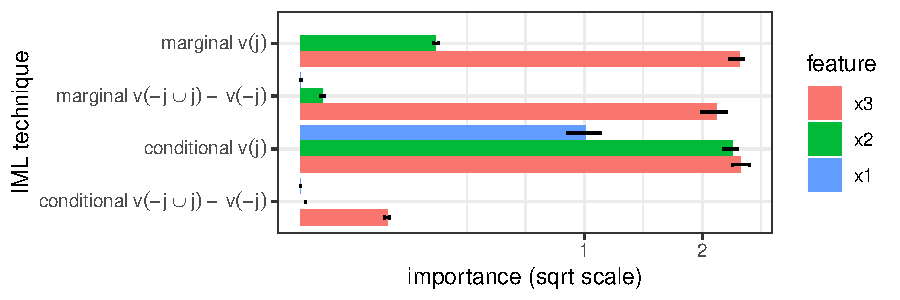
\includegraphics[width=\linewidth]{figure_man/sage_variants}}
\end{column}
\end{columns}
\lz
\begin{itemize}
    \item Marginal $v(j)$ are only nonzero for features that are used by $\fh$
    \item Conditional $v(j)$ are also nonzero for features that are not used by $\fh$ (e.g., due to correlation)
    \item For conditional value function $v$, the difference $v(-j \cup j) - v(-j)$ quantifies the unique contribution of $x_j$ over remaining features $x_{-j}$\\
    $\Rightarrow$ Since $y \indep x_1, x_2 | x_3$, only $v(\{1,2,3\}) - v(\{1, 2\})$ is nonzero (i.e., for feature $j = 3$)
\end{itemize}

\end{frame}


\begin{frame}{SAGE value functions versus SAGE values}

\textbf{SAGE value function $v(S)$}: measure contribution of a specific feature set over the empty coalition

\lz\pause

\textbf{SAGE values $\phi_j$}: fair attribution of importance
\begin{itemize}
    \item can be computed by averaging the contribution of $x_j$ over all feature orderings
    %\item for feature permutation $\pi$ and the corresponding feature ordering $(x_{\pi(1)}, \dots, x_{phi(d)})$, for feature $x_j$ the coalition $S(j; \pi)$ is defined as the set of features preceding $x_j$, i.e. $S(j; \pi) := \{i : \pi(i) < \pi(j)\}$
    %\item the contribution of $j$ in an ordering $\pi$ is given as $v(j \cup S(j; \pi)) - v(S(j; \pi))$
    \item for feature permutation $\tau$, the contribution of $j$ in the set $\Stau$ is given as $v(\Stauj) - v(\Stau)$\\
    Note: $\Stau$ is the set of features preceding $j$ in permutation $\tau$
\end{itemize}

\lz\pause

\textbf{SAGE value approximation:} Average over the contributions for $M$ randomly sampled permutations

\begin{align*}
    \phi_j = \frac{1}{M} \sum_{m=1}^M v(\Stauj) - v(\Stau)
\end{align*}
    
\end{frame}

\begin{frame}{Interaction Example Revisited}

\textbf{Recap:} Data: $x_1, \dots, x_4$ uniformly sampled from $\{-1, 1\}$ and $y:= x_1 x_2 + x_3 + \epsilon_Y$ with $\epsilon_Y \sim N(0, 1)$. Model: $\fh(x) \approx x_1 x_2 + x_3$.\\
%
\begin{figure}
  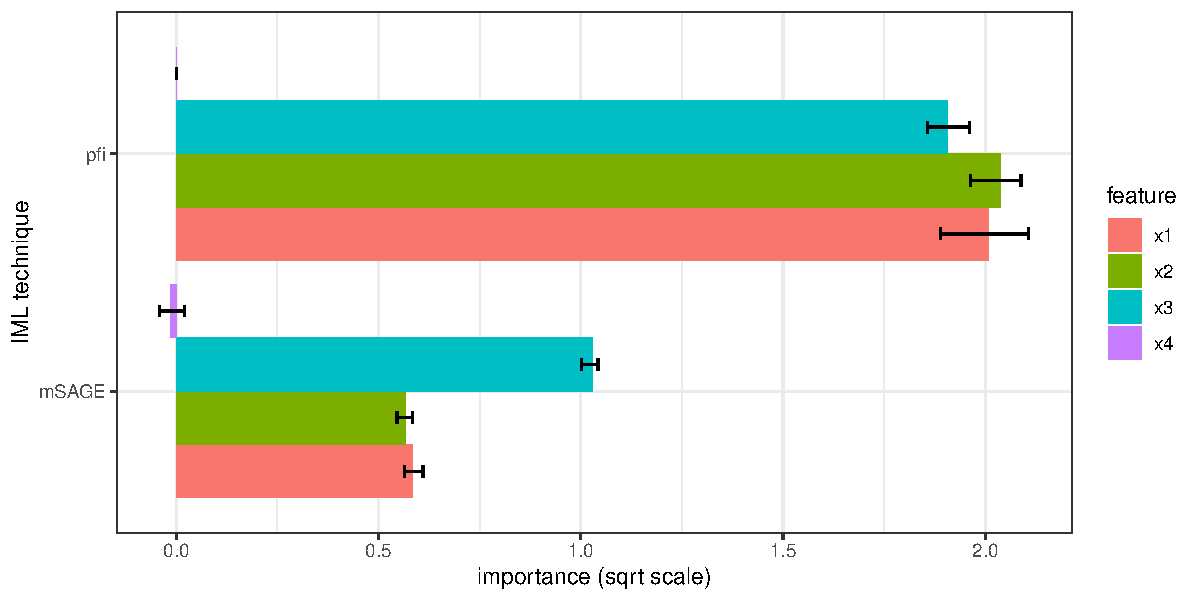
\includegraphics[width=0.65\linewidth]{figure_man/sage_pfi_interactions}
\end{figure}
%
\begin{itemize}
    \item PFI regards $x_1, x_2$ to be equally important as $x_3$
    \item Marginal SAGE fairly divides the contribution of the interaction $x_1$ and $x_2$
\end{itemize}

\end{frame}


\begin{frame}{SAGE Loss functions}

When the loss-optimal model $f^*$ is inspected using \textit{conditional-sampling} based SAGE value functions, interesting links exist.

\lz\pause
\textbf{For cross-entropy loss:} 
  \begin{itemize}
      \item value function is the mutual information:  $v_{f^*}(S) = I(y;x_S)$
      \item surplus contribution of a feature $x_j$ is the conditional mutual information: $v_{f^*}(S \cup \{j\}) - v_{f^*}(S) = I(y,x_i|x_S)$
  \end{itemize}

\lz\pause

\textbf{For MSE loss:} 
    \begin{itemize}
    \item value function is the expected reduction in variance given knowledge of the features $x_S$: $v_{f^*}(S) = Var(y) - \E[Var(y|x_S)]$
    \item surplus contribution is the respective reduction over $x_S$:
    $v_{f^*}(S \cup \{j\}) - v_{f^*}(S) = \E[Var(y|x_S)] - \E[Var(y|x_{S \cup {j}})]$
    \end{itemize}
    
\end{frame}


\begin{frame}{Implications marginal SAGE values}

Can we gain insight into whether the ...

\begin{enumerate}
    \item<1> feature $x_j$ is causal for the prediction?    \begin{itemize}
      \item for all coalitions $S$, $v(j \cup S) - v(S)$ can only be nonzero if $x_j \rightarrow \fh(x)$ (as for PFI)\\
      $\leadsto$ $\phi_j$ is only nonzero if $x_j$ is causal for the prediction
      \item $v(j \cup S) - v(S)$ may be zero due to independence $x_j \indep y | x_S$ (as for PFI)\\
      $\leadsto$ $\phi_j$ may be zero although the feature is causal for the prediction
    \end{itemize}
    \item<2> feature $x_j$ contains prediction-relevant information about $y$?
    \begin{itemize}
      \item value functions may be nonzero despite independence due to extrapolation (as for PFI)\\
      $\leadsto$ $\phi_j$ may be nonzero without $x_j$ being dependent with $y$
      \item value functions may be zero despite $x_j$ containing prediction-relevant information due to underfitting (as for PFI)\\
      $\leadsto$ $\phi_j$ may be zero although prediction-relevant information contained
    \end{itemize}
    \item<3> model requires access to $x_j$ to achieve it's prediction performance?    
    \begin{itemize}
      \item like PFI, in general marginal value functions do not allow insight into unique contribution $\leadsto$ no insight from $\phi_j$
    \end{itemize}
\end{enumerate}

\end{frame}
%
\begin{frame}{Implications conditional SAGE values}

Can we gain insight into whether the ...

\begin{enumerate}
    \item<1> feature $\xj$ is causal for the prediction?
    \begin{itemize}
      \item value functions may be nonzero although feature is not directly used by $\fh$\\
      $\leadsto$ nonzero $\phi_j$ does not imply $\xj \rightarrow \hat{y}$
      \item value functions may be zero although feature may be used by the model, e.g. if feature is independent with $y$ and all other features \\ $\leadsto$ zero $\phi_j$ does not imply $\xj \not \rightarrow \hat{y}$
    \end{itemize}
    \item<2> feature $\xj$ contains prediction-relevant information about $y$?
    \begin{itemize}
      \item e.g. for cross-entropy optimal $\fh$, $v(j)$ measures mutual information $I(y;x_j)$
      $\leadsto$ prediction-relevance implies nonzero $\phi_j$
      \item $x_j \indep y$ does not imply $x_j \indep y | x_S$ and consequently does not imply $v(j \cup S) - v(S) = 0$
      $\leadsto$ $\phi_j$ may be nonzero although $\xj \indep y$
    %   \item $x_j \indep y$ in general does not imply $x_j \indep y | x_S$ and consequently does not imply that $v(j \cup S) - v(S) = 0$\\
    %   $\leadsto$ $\phi_j$ may be nonzero although $\xj \indep y$
    \end{itemize}
    \item<3> model requires access to $x_j$ to achieve it's prediction performance?  
    \begin{itemize}
        \item e.g. for cross-entropy optimal $\fh$, the surplus contribution $v(j \cup -j) - v(-j)$ captures the conditional mutual information $I(y;x_j|x_{-j})$\\
        $\leadsto$ $\phi_j$ is nonzero for features with unique contribution
        \item $x_j \indep y | x_{-j}$ does not imply $x_j \indep y | x_S$ (cond. w.r.t. to arbitrary coalitions $S$)\\
        $\leadsto$ $\phi_j$ may be nonzero although the features has no unique contribution
    \end{itemize}
\end{enumerate}

\end{frame}

% \begin{frame}
%   \printbibliography
% \end{frame}

\begin{frame}{Deep dive: Shapley axioms for SAGE}

The Shapley axioms can be translated into properties of SAGE. The interpretation depends on whether conditional or marginal sampling is used.
%
\begin{table}
  \centering
  \begin{tabular}{l | l }
  Shapley property $\implies$ & conditional SAGE property \\
  \hline
  efficiency & $\sum_{i=1}^p \phi_j(v) = \risk(\fh_\emptyset) - \risk(\fh)$\\
  symmetry & $x_j = x_i \implies \phi_i = \phi_j$ \\
  linearity & $\phi_j$ expecation of per-instance\\
  & conditional SHAP applied to model loss\\
  monotonicity & given models $f, f'$, if  $\forall S:$\\
  &$v_f(S \cup j) - v_f(S) \geq v_{f'}(S \cup j) - v_{f'}(S)$ \\
  &then $\phi_j(v_f) \geq \phi_j(v_{f'})$\\
  dummy & if $\forall S: \fh(x) \indep x_j | x_S \Rightarrow \phi_j = 0$
  \end{tabular}
\end{table}

\end{frame}

\begin{frame}{Deep dive: Shapley axioms for SAGE}
%
The Shapley axioms can be translated into properties of SAGE. The interpretation depends on whether conditional or marginal sampling is used.
%
\begin{table}
  \centering
  \begin{tabular}{l | l }
  Shapley property $\implies$ & marginal SAGE property \\
  \hline
  efficiency & $\sum_{i=1}^p \phi_j(v) = \risk(\fh_\emptyset) - \risk(\fh)$\\
  symmetry & no intelligible implication \\
  linearity & $\phi_j$ expecation of per-instance\\
  & marginal SHAP applied to model loss\\
  monotonicity & given models $f, f'$, if  $\forall S:$\\
  &$v_f(S \cup j) - v_f(S) \geq v_{f'}(S \cup j) - v_{f'}(S)$ \\
  &then $\phi_j(v_f) \geq \phi_j(v_{f'})$\\
  dummy & model invariant to $x_j \Rightarrow \phi_j = 0$\\
  \end{tabular}
\end{table}
%
\end{frame}

\endlecture
\end{document}
